With the last experiment we found the bare resonator frequency (also called \textit{high power frequency}), but this is not the frequency that will be used in measurements.
We need to find the frequency in the low power regime, where the resonator is actually coupled to the qubit~\cite{Gao2008}.
To do that, we first have to find the correct amplitude of the readout pulse.

Also this experiment can be initially performed with a VNA, to check everything is working and to obtain a rough estimation of the parameters to be used by the control devices.

We do again a resonator spectroscopy experiment, measuring at different frequencies, but this time scanning in a narrow frequency span and also for different pulse amplitudes.
We expect the resonator frequency to have a strong dependency on the amplitude: in particular we expect it to be fixed at first (in the high power regime) then undergo a transition phase and then be fixed again at a different frequency because of the coupling with the qubit.
Eventually, we want to have a plot like \cref{fig:punchout_sketch}

\begin{figure}[ht]
    \makebox[\textwidth][c]{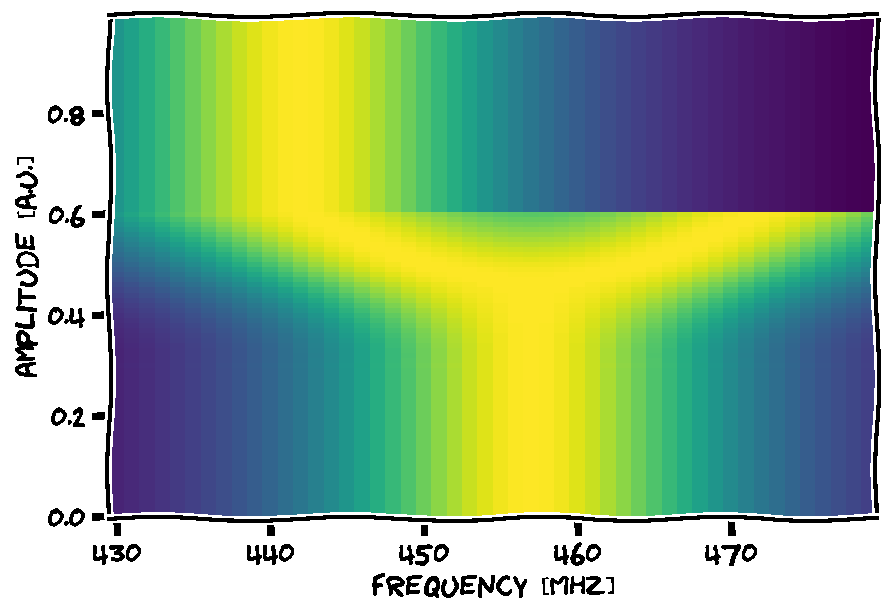
\includegraphics[width=8cm]{characterization/figures/resonator_punchout_sketch.pdf}}
    \caption{Expected plot for a resonator punchout experiment. From this we could choose an amplitude of $0.3$ at $\approx 480$ MHz.}
    \label{fig:punchout_sketch}
\end{figure}

This experiment is the first one where we actually are "seeing" the qubit and it is extremely important also to check that the qubit is working properly.
During a characterization, various experimental problems can happen and can lead the experimenter to believe that the qubit is no longer working: this experiment gives us an easy way to check it.

Moreover, from this experiment we can actually already have an estimate of the qubit frequency~\cite{Majer2007, Roth2021, Gu2017} using:
\begin{equation}
    \omega_{rh} - \omega_{rl} = \chi = \frac{g^2}{\Delta}
\end{equation}
Where $\Delta=\omega_{rl} - \omega_q$.

So, if we know, maybe from design specifications, the expected value of $g$, we can have an estimate of the qubit frequency.
If, as in most cases, we do not have information on $g$, than we still can infer if the qubit frequency is higher or lower than the resonator frequency.

To obtain a clear plot, this experiment usually requires multiple tries, to choose "good parameters".
In particular:
\begin{itemize}
    \item the amplitude range and step must be chosen carefully because punchout can lead to extremely long experiments (that we would like to avoid), but large steps will inevitably confuse the plot;
    \item the frequency usually shifts very little, but depending on $g$ and $\Delta$, so it is difficult to set the frequency span and step;
    \item if the scan in amplitude is linear, it will be difficult to have a clear view of all the three regimes at the same time. If it is possible, it may be worth to do a logarithmic scan.
\end{itemize}

Note also that, in literature, this plot is often presented as a scan in the \textit{attenuation} of the readout line.
The effect is the same as of changing the amplitude (although it is by default a logarithmic scan), but the plot is reversed: at the top (high attenuation) we will see the low power regime and at the bottom (low attenuation) the high power one.

In \cref{fig:punchouts} different punchout plots are shown, so that is understandable how much they can differ.
Note that "the colors are normalized" for every amplitude and we actually have very high amplitudes in high power, and much lower amplitude elsewhere.
\begin{figure}[ht]
    \centering
    \subfloat[\centering Resonator punchout for a cavity.]{
        \makebox[\textwidth][c]{
        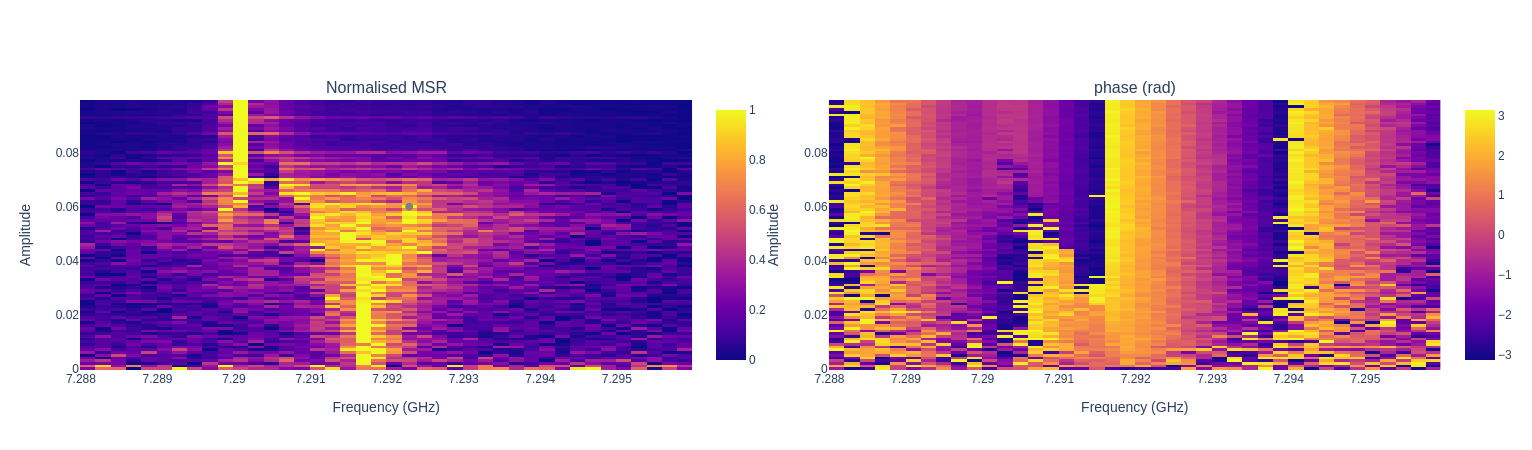
\includegraphics[width=1.3\textwidth]{characterization/figures/punchout.png}}
    }\\
    \subfloat[\centering Resonator punchout for a 2D resonator.]{
        \makebox[\textwidth][c]{
        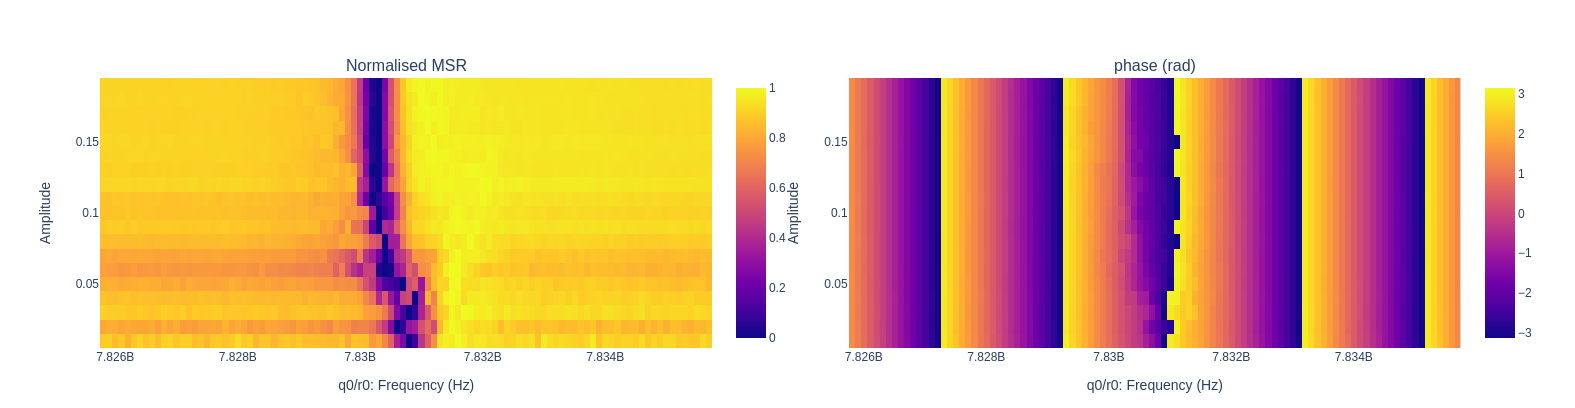
\includegraphics[width=1.3\textwidth]{characterization/figures/res_punchout_2.png}}
    }
    \caption{Different plots for the resonator punchout experiment.}
    \label{fig:punchouts}
\end{figure}

From these plots we can extract few things: first of all, the pulse  amplitude that we will use for the next experiments for the readout pulse.
We should try to use the amplitude that maximize the S/N ratio for the resonator, so in general the highest amplitude at low power.
However, we still need to be sure to not enter the transition regime, something that could lead to very noisy experiments and eventually prevent us to reach any sensible result.
To be sure that, at the given pulse amplitude, we are not in the transition regime, we can repeat the standard resonator spectroscopy with a finer scan, checking if the peak is Lorentzian.\\
A resonator spectroscopy is also useful to better check the resonator frequency at low power that will present with a lower quality factor as shown in \cref{fig:resonator_spectroscopy_after_punchout}.

\begin{figure}[ht]
    \makebox[\textwidth][c]{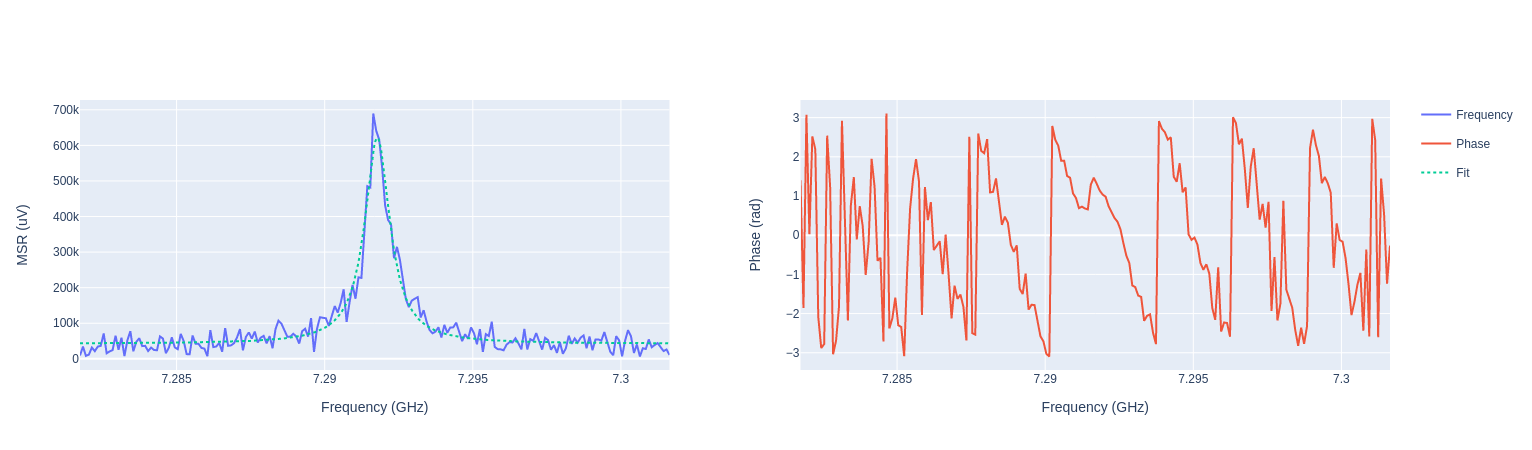
\includegraphics[width=1.3\textwidth]{characterization/figures/resonator_3D_low_power.png}}
    \caption{Resonator spectroscopy of a 3D cavity in the low power regime.}
    \label{fig:resonator_spectroscopy_after_punchout}
\end{figure}

Last but not least, we can write down also the maximum value of the peak.\\
Since we are not interacting directly with the qubit, we are effectively measuring the amplitude of the ground state and, from now on we will not change the resonator frequency, so we expect to always measure this amplitude for the zero state.
Here it is not needed to do a precise measurement, but it is nevertheless very useful to have an approximate value, that can later be used to check, in other experiments, that we are not exciting the qubit by error (if we see a change in amplitude, then maybe the qubit state has changed).

\experimentrecap
{Resonator punchout}
{readout calibration}
{amplitude for the readout pulse,\\frequency of the resonator in low power (frequency of readout),\\signal amplitude for qubit ground state,\\estimation of the qubit frequency}
{a measurement is executed with pulses of different frequencies and amplitude. We do a 3D plot with transmitted signal vs frequency vs amplitude. We extract amplitude and frequency for low power regime. We estimate the qubit frequency and the signal amplitude of the qubit ground state}